\documentclass[a4paper,11pt,BCOR10mm,oneside,headsepline]{scrartcl}
\usepackage{amsmath, mathtools}
\usepackage[ngerman]{babel}
\usepackage[utf8]{inputenc}

\usepackage{typearea, url}
\areaset{17cm}{26cm}
\setlength{\topmargin}{-1cm}
\usepackage{scrpage2}
\pagestyle{scrheadings}

\usepackage[T1]{fontenc}
\usepackage{beramono}
\usepackage{listings}
\usepackage[usenames,dvipsnames]{xcolor}
\usepackage{graphicx}
\usepackage{subcaption}

\ihead{HW5: CIS 631, Parallel Processing}
\ohead{\pagemark}
\chead{}
\cfoot{}

\begin{document}
	
	\begin{center}
		\textbf{\large Homework 5 Report}
	\end{center}\vskip1em
	
	\section{Test Environment}
	I tested my code on a Google Compute Instance with NVIDIA Tesla V100 GPU, with CUDA 11.1.
		
	\section{Experiments and Results}
	\subsection{CSR Scalar}
			Each block contains \(T\) threads. The grid is divided into \(m\) blocks.
			\begin{figure}[!htbp]
				\centering
				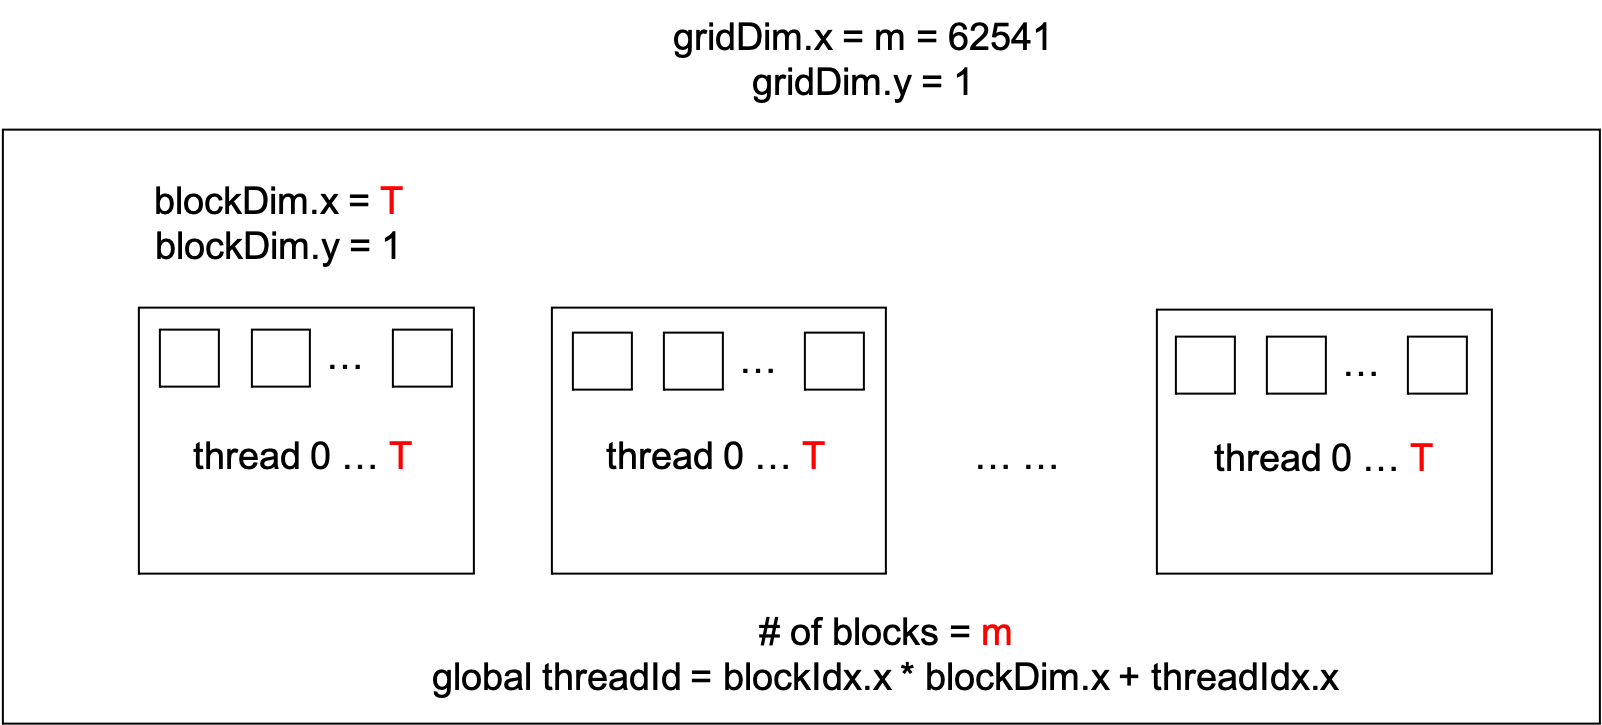
\includegraphics[scale=0.5]{./figures/csr_scalar}
				\caption*{Figure 1. CSR Scalar: Divide Grid into Blocks}
			\end{figure}
			
			Experiment result for m blocks, each block contain 32, ... , 1024 threads.
			\begin{figure}[!htbp]
				\centering
				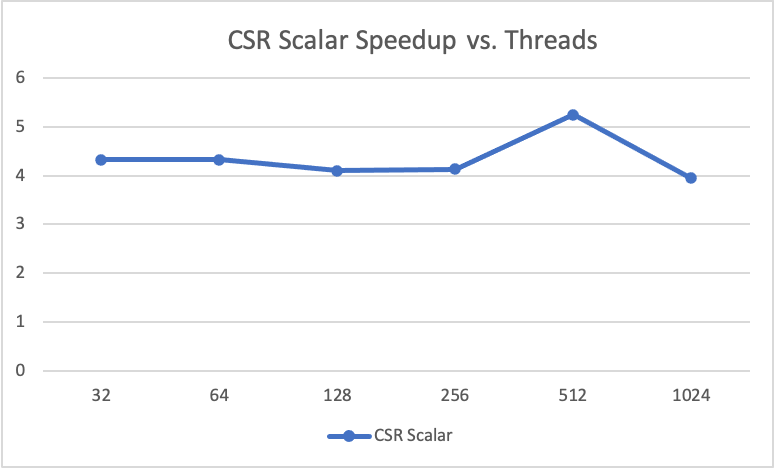
\includegraphics[scale=0.6]{./figures/csr_scalar_result}
				\caption*{Figure 2. CSR Scalar: Experiment Results}
			\end{figure}
	
		\newpage
		\subsection{CSR Vector Reduction with Shared Memory}
		This uses reduction. Each block contains \(T\) threads. The grid is divided into m blocks. An array is declared as share memory to store intermediate results. Syncthreads() is called when calculate local sums and reduce local sums to global sum.
		
		\begin{figure}[!htbp]
			\centering
			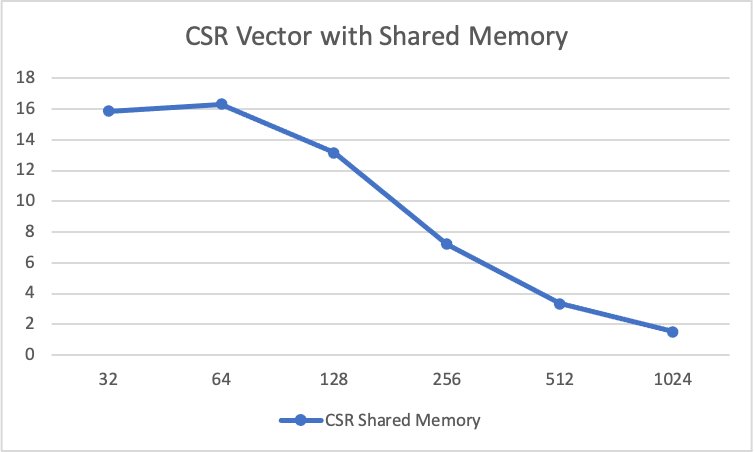
\includegraphics[scale=0.6]{./figures/csr_shared_result}
			\caption*{Figure 3. CSR Vector with Shared Memory: Result}
		\end{figure}
		
		\subsection{ELL without Shared Memory}
		I implemented ELL similar to CSR scalar. Each block contains \(T\) threads. The grid is divided into \(m\) blocks.
		
		\begin{figure}[!htbp]
			\centering
			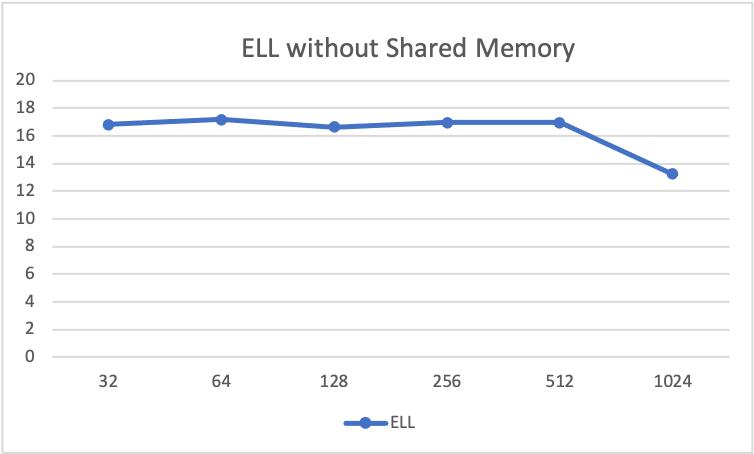
\includegraphics[scale=0.5]{./figures/ell_result}
			\caption*{Figure 4. Ell without Shared Memory: Result}
		\end{figure}
	
		\subsection{ELL with Shared Memory}
		This is similar to CSR reduction with shared memory.
		
		\begin{figure}[!htbp]
			\centering
			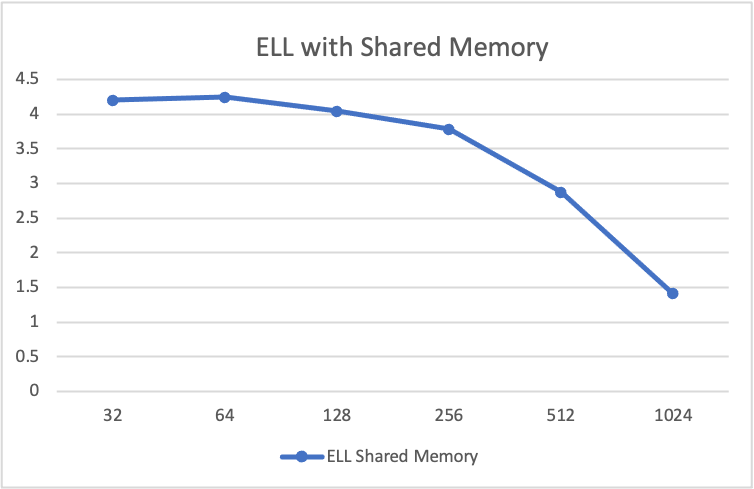
\includegraphics[scale=0.5]{./figures/ell_shared_result}
			\caption*{Figure 5. Ell with Shared Memory: Result}
		\end{figure}
		
		\newpage
		\subsection{Performance Comparison}
			\begin{figure}[!htbp]
				\centering
				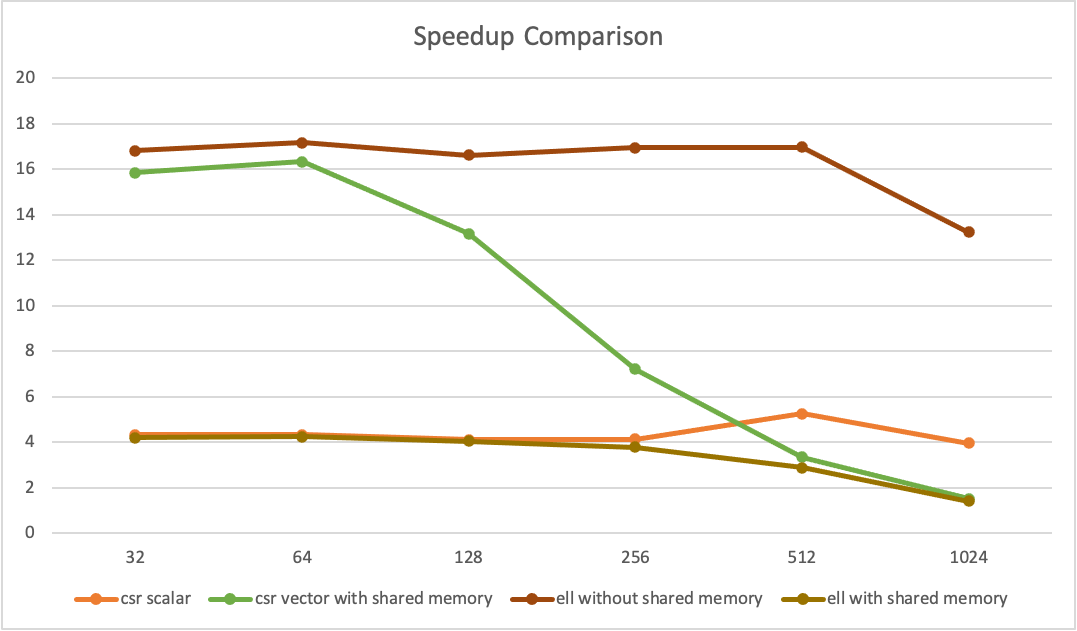
\includegraphics[scale=0.5]{./figures/comparison}
				\caption*{Figure 6. Performance Comparison}
			\end{figure}

	\section{Findings}
		\begin{itemize}
			\item The best performance is achieved by ELL without shared memory, which gains 17.16x speedup than CPU SPMV.
			\item CSR scalar implementation has some problems that led to poor performance. Since adjacent threads cannot access data in a contiguously way, the hardware cannot combine memory access for concurrent threads.
			\item CSR vector implementation addresses the problems that CSR scalar has. CSR vector accesses indices and data contiguously, and overcomes the problem of load balancing and memory access pattern.
			\item ELL addresses non-coalesced memory access of CSR by using padding and transposition on the sparse matrix. By allowing coalesced memory access, ELL outperforms CSR.
			\item ELL shared memory performs worse than without shared memory. This is most likely due to the fact that ELL already has a coalesced memory access pattern, by doing reduction with shared memory will cause more overhead.
		\end{itemize}
	
\end{document}